Description of the problem ($\FP+\CC+\MA+\BW$).

\subsection{Dynamic programming on trees}

Intro to dynamic programming on trees with subtree decomposition.
Introduce binarization as way of dealing with trees of larger arity.
Mention correctness requirements: substructure optimality and overlapping subproblems.

\subsection{Introduction to our algorithm}

We will want to go through all VM placements, for each of those do greedy matching and choose the cheapest.

Solution for subtree - how it can look like? It is ``partial matching''. Some matched VMs and chunks, but also some chunks transported out of subtree or some VMs/slots that will have chunks transported into from outside. So we charge already those incomplete matchings.

Cost charging model - two edges. Recursive formula for calculating the cost - the $f$ function. \maciek{I had the early sketch of definition of $f$ somewhere, but it was deleted or commented out and I cannot find that.}

Recursive formula for cost with bandwidth. 

\subsection{Algorithm}

TODO: hosting multiple VMs in the same node

List all needed functions like distance, counter of number of chunks in subtree.

Present the pseudocode, with base cases, aggregate function.

Tell how to go back through the array to reconstruct the actual placements. ``Following path of minimas''.
Note that it computationally intensive, and we can trade it for memory - we can remember the best placement.

\subsection{Algorithm correctness}
\subsubsection{Optimality of greedy matching}

For general complete bipartite graphs the matching constructed by greedily choosing the cheapest edge can be arbitrarily bad.
However, in case of very specific graph, where weights are induced by distance in a tree, this strategy produces optimal solution.
By using properties of the tree, we will show following lemma:

\begin{lemma}
  Given fixed positions of VMs, the local greedy perfect matching of chunks to VMs inclines minimal cost among all possible perfect matchings.
\end{lemma}

\begin{proof}
Proof by contradiction. Let's assume that there exists matching of cost lower than cost of $G$. Let's take cheapest such matching and call it $H$.

Let's find smallest subtree $S$ where partial matching of $G$ has different cost than partial matching of $H$. It means that in both left and right subtree we did local matching (do we need this sentence?). It means that non-local decision was made in this subtree (perhaps hoping for savings higher?). Then there exist two such two such matched pairs in $H$ that shares an edge (one pair is transporting chunk up, the second one is transporting chunk down). Then we can create matching $H'$ that uncrosses those edges (does the local matching on them) and is cheaper than $H$. Contradiction.


\maciek{It means basically that in every subtree we can only have more costly solution. Perhaps there exist cleaner way of proving that.}
\end{proof}


\subsubsection{Bandwidth correctness.}

\begin{lemma}
Let's say that we calculated solution for our instance of VC with ignoring the bandwidth. Then we analyzed every link and it turned out that some of them exceed their capacity. Then the instance is infeasible and we cannot fix that by choosing any other matching (even suboptimal one).
\end{lemma}

It might happen that this lemma does not hold, beware!

\maciek{Below there is emergency lemma in case that above lemma does not hold. In case above lemma is true it implies that below lemma is true.}
\begin{lemma}
An instance of $\Problem$ is infeasible iff. algorithm returns $\infty$.
\end{lemma}
\begin{proof}
  ($\rightarrow$)

  ($\leftarrow$)
  \end{proof}

\maciek{I think that we do not need that lemma, it might be obvious. I leave it there just in case.}
\begin{lemma}
  If algorithm returns solution $\Sol$ of cost $\neq \infty$, then in $\Sol$ no link exceeds its capacity limit.
  \end{lemma}

\subsubsection{Substructure optimality without bandwidth.}

Definition of partial matching (matching + transporting imbalanced chunks out of tree and transporting chunk into imbalanced VMs from outside the tree). Definition of partial matching optimality (parametrized by number of VMs, subtree and chunks; best among all possible that match the same chunks and transports the imbalance).

\begin{lemma}
(uplink lemma)
For every tree T (with chunks) and number of VMs $x$ the bandwidth of uplink is the same among all possible feasible solutions (\maciek{it is the lemma that Carlo formulated})

\maciek{unless we allow something as stupid as routing communication and transport through loops}
\end{lemma}

\begin{lemma}

Let's consider an arbitrary tree $T$ with chunks $c_i$ and number of VMs $v$. Than $f(T, v)$ is cost of optimal partial matching.

\end{lemma}

\begin{proof}
Proof by structural induction. First, we take definition of $f$, which contains values of $f$ for left and right subtree for different number of VMs (but which sum to $v$). We can assume by induction that those are optimal. Then we calculate the cost of communication and matching between left and right subtree (also in $f$'s definition. Then we choose the minimum cost one. We argue that this one is optimal partial matching, and we use optimality of greedy matching for that.

Also, we use the uplink lemma to show that choosing optimal partial matching in left and right subtree does not generate excessive bandwidth on both uplink edges (we might have doubted that because optimal partial matchings were restricted to their subtrees and we might thought that there is some other more costly matching that has less bandwidth on uplink - to save there).
\end{proof}

\subsubsection{Substructure optimality with bandwidth.}
\subsection{Running time and memory consumption analysis}

\begin{figure}
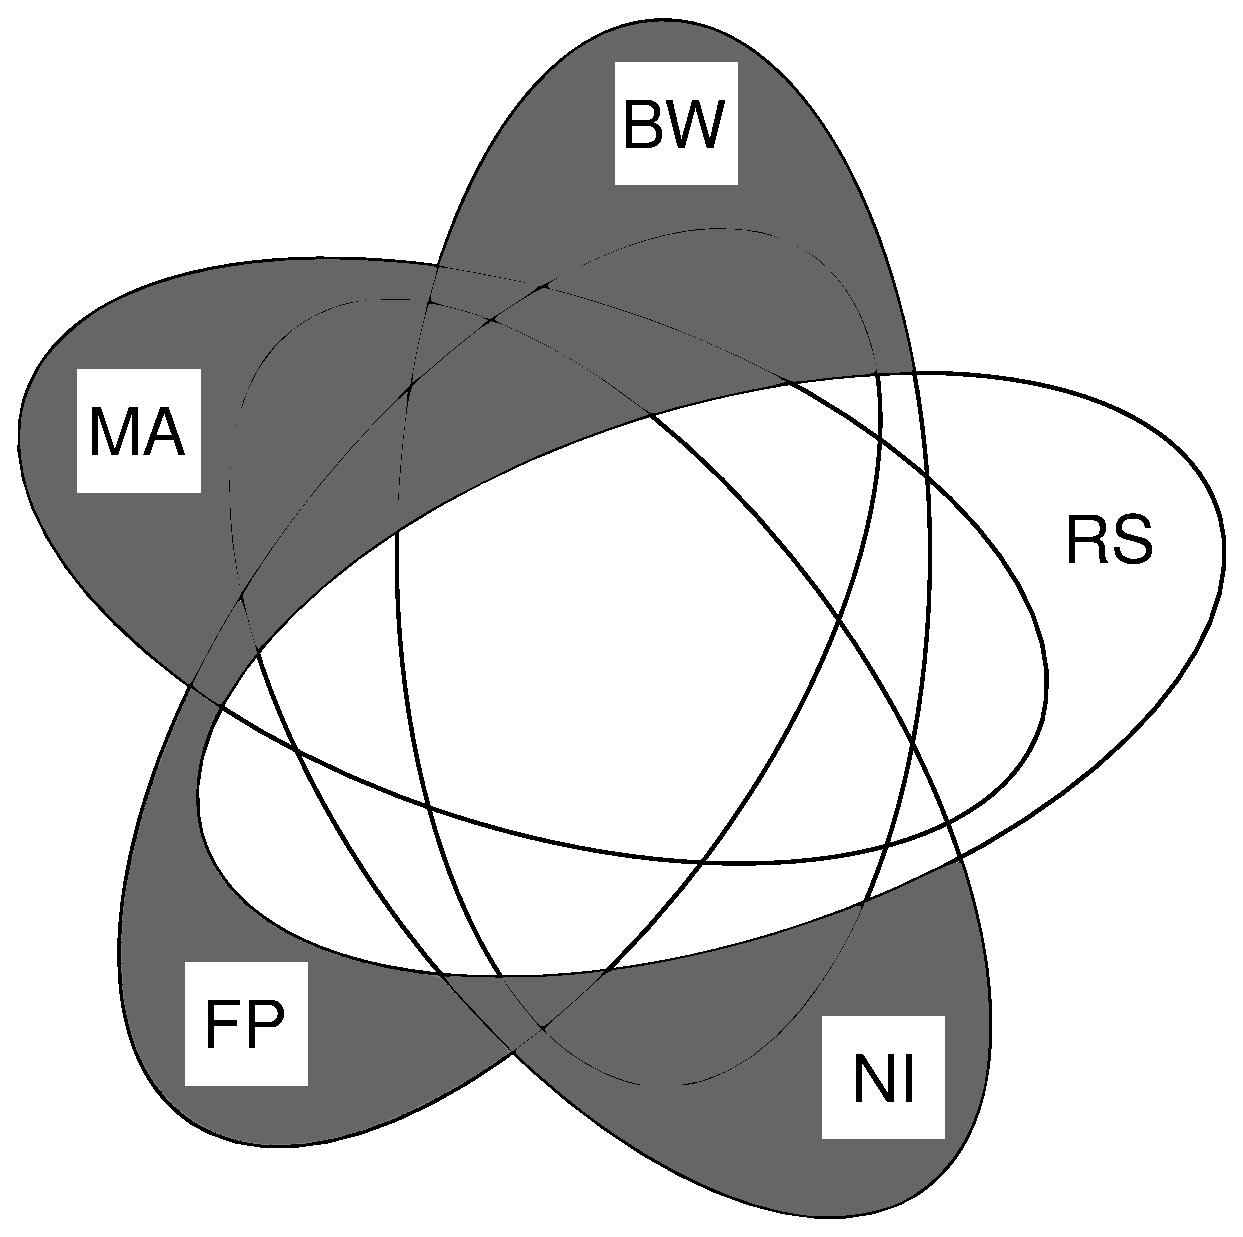
\includegraphics[width=\columnwidth]{figs/venn_dp.pdf}
\caption{Property combinations which can be solved by our dynamic prorgramming 
appraoch.}
\label{fig:venn_dp}
\end{figure}

\carlo{Figure~\ref{fig:venn_dp} shows illustrates which problem 
combiantions can be solved by the presented dynamic programming approach.}
